\PassOptionsToPackage{unicode=true}{hyperref} % options for packages loaded elsewhere
\PassOptionsToPackage{hyphens}{url}
%
\documentclass[]{article}
\usepackage{lmodern}
\usepackage{amssymb,amsmath}
\usepackage{ifxetex,ifluatex}
\usepackage{fixltx2e} % provides \textsubscript
\ifnum 0\ifxetex 1\fi\ifluatex 1\fi=0 % if pdftex
  \usepackage[T1]{fontenc}
  \usepackage[utf8]{inputenc}
  \usepackage{textcomp} % provides euro and other symbols
\else % if luatex or xelatex
  \usepackage{unicode-math}
  \defaultfontfeatures{Ligatures=TeX,Scale=MatchLowercase}
\fi
% use upquote if available, for straight quotes in verbatim environments
\IfFileExists{upquote.sty}{\usepackage{upquote}}{}
% use microtype if available
\IfFileExists{microtype.sty}{%
\usepackage[]{microtype}
\UseMicrotypeSet[protrusion]{basicmath} % disable protrusion for tt fonts
}{}
\IfFileExists{parskip.sty}{%
\usepackage{parskip}
}{% else
\setlength{\parindent}{0pt}
\setlength{\parskip}{6pt plus 2pt minus 1pt}
}
\usepackage{hyperref}
\hypersetup{
            pdftitle={Statistical analysis of periodic data in neuroscience},
            pdfauthor={Daniel H. Baker},
            pdfborder={0 0 0},
            breaklinks=true}
\urlstyle{same}  % don't use monospace font for urls
\usepackage[margin=1in]{geometry}
\usepackage{longtable,booktabs}
% Fix footnotes in tables (requires footnote package)
\IfFileExists{footnote.sty}{\usepackage{footnote}\makesavenoteenv{longtable}}{}
\usepackage{graphicx,grffile}
\makeatletter
\def\maxwidth{\ifdim\Gin@nat@width>\linewidth\linewidth\else\Gin@nat@width\fi}
\def\maxheight{\ifdim\Gin@nat@height>\textheight\textheight\else\Gin@nat@height\fi}
\makeatother
% Scale images if necessary, so that they will not overflow the page
% margins by default, and it is still possible to overwrite the defaults
% using explicit options in \includegraphics[width, height, ...]{}
\setkeys{Gin}{width=\maxwidth,height=\maxheight,keepaspectratio}
\setlength{\emergencystretch}{3em}  % prevent overfull lines
\providecommand{\tightlist}{%
  \setlength{\itemsep}{0pt}\setlength{\parskip}{0pt}}
\setcounter{secnumdepth}{5}
% Redefines (sub)paragraphs to behave more like sections
\ifx\paragraph\undefined\else
\let\oldparagraph\paragraph
\renewcommand{\paragraph}[1]{\oldparagraph{#1}\mbox{}}
\fi
\ifx\subparagraph\undefined\else
\let\oldsubparagraph\subparagraph
\renewcommand{\subparagraph}[1]{\oldsubparagraph{#1}\mbox{}}
\fi

% set default figure placement to htbp
\makeatletter
\def\fps@figure{htbp}
\makeatother


\title{Statistical analysis of periodic data in neuroscience}
\author{Daniel H. Baker}
\date{13/12/2020}

\begin{document}
\maketitle

\hypertarget{abstract}{%
\section{Abstract}\label{abstract}}

Many experimental paradigms in neuroscience involve driving the nervous system with periodic sensory stimuli. Neural signals can then be recorded, and include phase-locked oscillations at the stimulation frequency. The analysis of such data often involves standard univariate statistics such as T-tests, conducted on the Fourier amplitude components. However, the assumptions of these tests will often be violated because amplitudes are not normally distributed, and weak signals might be missed if the phase information is discarded. An alternative approach is to conduct multivariate statistical tests using the real and imaginary Fourier components. Here we compare the performance of two multivariate extensions of the T-test, Hotelling's \(T^2\) and a variant called \(T^2_{circ}\). We develop a novel test of the assumptions of \(T^2_{circ}\) based on the condition index, and a heuristic for excluding outliers using the Mahanalobis distance. We then extend the statistic to multi-level designs, and propose a new statistical test termed \(ANOVA^2_{circ}\). This has identical assumptions to \(T^2_{circ}\), and is shown to be more sensitive than MANOVA when these assumptions are met. We demonstrate how these tests might be applied to two publicly available empirical data sets, and suggest concrete guidance for choosing which test to run. Implementations of these novel tools are provided as \emph{R} functions, and we hope that their wider adoption will improve the sensitivity of statistical inferences involving periodic data.

\hypertarget{background}{%
\section{Background}\label{background}}

A widely used paradigm in many branches of neuroscience is to drive the nervous system using periodic stimuli. This entrains neural responses at the stimulation frequency, resulting in high signal-to-noise ratios relative to single stimulus presentations. These periodic responses, often called the \emph{steady-state} or \emph{frequency following} response, can be recorded from single neurons (Enroth-Cugell and Robson 1966) and local field potentials (Morrone, Burr, and Speed 1987) using invasive methods, or with non-invasive electroencephalography (EEG) and magnetoencephalography (MEG) systems, both in humans (Norcia et al. 2015) and in diverse animal species including insects (Afsari et al. 2014), birds (Porciatti et al. 1990), rodents (Hwang et al. 2019) and primates (Nakayama and Mackeben 1982). Steady-state methods are used to measure early sensory responses in vision (Regan 1966), hearing (Rees, Green, and Kay 1986) and somatosensation (Snyder 1992), and closely related paradigms have been developed to target specific stimulus features such as orientation (Braddick, Wattam-Bell, and Atkinson 1986), and facial expression (Gray et al. 2020) and identity (Liu-Shuang, Norcia, and Rossion 2014). In fMRI research, \emph{travelling wave} methods (Engel et al. 1994; Sereno et al. 1995) are used to map the retinotopic responses of early visual cortex using stimuli that change periodically in spatial position. Finally, physiological reflexes such as the pupillary response to light can be entrained in a similar way (Spitschan et al. 2014).

A convenient way to analyse the data from periodic stimulation experiments is to take the Fourier transform of the measured signal. The amplitude of the response at the stimulation frequency (and its harmonics - integer multiples of the stimulation frequency) is a convenient, and well-isolated index of the brain's response. Fourier spectra comprise both amplitude and phase information, which can be equivalently expressed as complex numbers with real and imaginary components. In many studies the phase information is routinely discarded, and statistical comparisons are performed on the amplitude data only. However an alternative is to use multivariate statistics, which take into account both the amplitude and phase information (represented as real and imaginary components). Multivariate methods have the advantage that they are more sensitive to weak signals, and therefore offer increased statistical power relative to univariate methods.

For pointwise and pairwise comparisons, Hotelling's \(T^2\) statistic (Hotelling 1931) is a multivariate extension of the T-test. For the one-sample case, the test statistic is defined as:

\begin{equation}
\label{eq:t2eq}
T^2 = N(\bar{x} - \mu)' C^{-1} (\bar{x} - \mu),
\end{equation}

where \emph{N} is the number of observations, \(\bar{x}\) is the multivariate sample mean, \(\mu\) is the point of comparison, \(C^{-1}\) is the inverse covariance matrix, and \('\) denotes vector transposition. Conceptually, the \(T^2\) statistic extends the univariate T-statistic by incorporating the covariance between the dependent variables. Two-sample and paired variants are also available, and the test can be applied to an arbitrary number of dependent variables (though here we will consider only the bivariate case).

More recently, Victor and Mast (1991) proposed a simpler version of \(T^2\), called \(T^2_{circ}\). The \(T^2_{circ}\) statistic makes the strong assumption that the dependent variables (real and imaginary values) are uncorrelated and have equal variance. When these conditions are met, the test statistic is defined as:

\begin{equation}
\label{eq:t2c}
T^2_{circ} = (N-1)\frac{|\bar{x}-\mu|^2}{\Sigma|x_j - \bar{x}|^2}
\end{equation}

where \(x_j\) denotes the \(j\)th observation of the dependent variables, and all other terms retain their previous meanings. Notice that no covariance term is present in equation \eqref{eq:t2c}, because of the independence assumption. This makes the statistic simpler to calculate, but causes problems when the assumption is violated.

In the present paper, we develop best practice guidelines for performing statistical tests on multivariate Fourier components derived from periodic stimulation paradigms. We first demonstrate why parametric univariate statistics are inappropriate for such data, because amplitudes for weak signals are not normally distributed. We then investigate conditions under which we should use either the \(T^2\) or \(T^2_{circ}\) statistic. The range of sample sizes and effect sizes where \(T^2_{circ}\) is more sensitive is identified. We develop a novel method for testing the assumptions of the \(T^2_{circ}\) statistic, based on calculating the condition index of a multivariate data set. Appropriate methods for identifying outliers using the Mahalanobis distance are discussed, and a heuristic proposed. Next the logic of \(T^2_{circ}\) is extended to situations with more than two levels of the independent variable, and the performance of this novel \(ANOVA^2_{circ}\) statistic is compared to MANOVA. Finally, we demonstrate the proposed techniques on two example SSVEP data sets, and recommend some best practice guidelines for analysis decisions.

All scripts used to generate this manuscript are available at: \url{https://github.com/bakerdh/FourierStats}. These include \emph{R} functions to implement one-sample Hotelling's (1931) \(T^2\) statistic, Victor \& Mast's (1991) \(T^2_{circ}\) statistic, and the condition index and \(ANOVA^2_{circ}\) statistics proposed in this paper.

\hypertarget{fourier-amplitudes-violate-parametric-assumptions-of-univariate-statistics}{%
\section{Fourier amplitudes violate parametric assumptions of univariate statistics}\label{fourier-amplitudes-violate-parametric-assumptions-of-univariate-statistics}}

Many empirical studies use univariate T-tests or analysis of variance (ANOVA) to analyse periodic data. Specifically, the amplitude component of the Fourier spectrum at the stimulation frequency is used as the dependent variable, discarding the phase information. This is problematic, because the amplitude is an absolute quantity, and can never fall below zero. Distributions of amplitudes for weak signals are therefore positively skewed, and will generally violate the assumption of normality.

\begin{figure}

{\centering 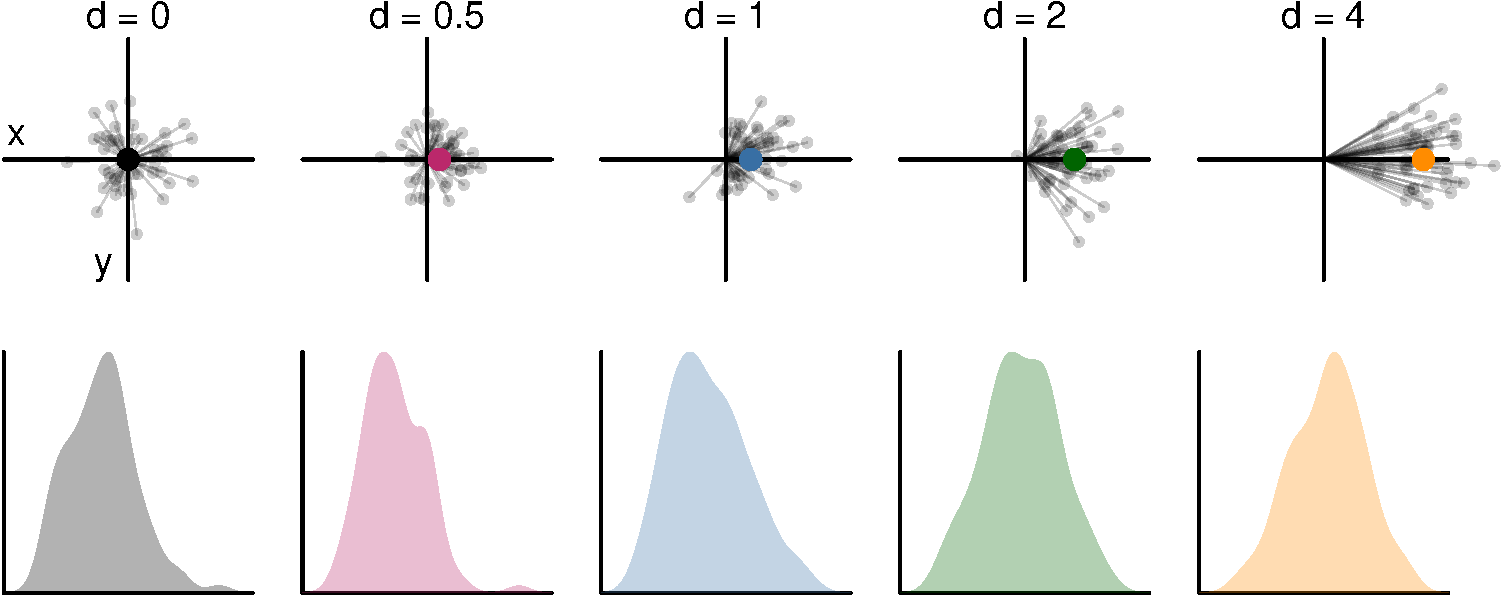
\includegraphics{manuscript_files/figure-latex/amphists-1} 

}

\caption{Demonstration of skew in absolute Fourier amplitudes for weak signals. Signal strength is quantified as Cohen's d, defined as the ratio of the mean to the standard deviation of the sample. The upper row shows samples of 50 grey points, and the population mean (coloured points). The lower row shows kernel density functions generated from 100,000 amplitude values. Note that the mean phase of the signal is irrelevant for these simulations, and is shown in the positive x-direction for consistency.}\label{fig:amphists}
\end{figure}

The upper row of Figure \ref{fig:amphists} shows scatterplots of simulated Fourier components, expressed using real (x) and imaginary (y) components. The amplitudes are the lengths of the lines joining each grey point to the origin. The lower row in Figure \ref{fig:amphists} shows distributions of amplitudes for the same set of signal strengths. These distributions only approach normality when the signal strength is more than twice the standard deviation (Cohen's d \textgreater{} 2; Cohen's d is the mean difference scaled by the standard deviation, see Cohen (1988)). One consequence of this is that T-tests will potentially have an inflated Type 1 error (false positive) rate for many signals encountered empirically.

Typical solutions, such as log-transforming the data, are unlikely to be equally applicable to all conditions. For example, if one wishes to compare a baseline where no stimulus was presented with a condition involving a strong signal, the former will be skewed and the latter normal. Applying a transform to both conditions is therefore problematic. Non-parametric statistics are a potential option, but these have generally lower statistical power than their parametric equivalents. Instead, the bivariate statistics discussed in the introduction avoid these issues and have greater statistical power, and should be used in preference to univariate methods.

\hypertarget{conditions-under-which-t2_circ-is-more-sensitive-than-t2}{%
\section{\texorpdfstring{Conditions under which \(T^2_{circ}\) is more sensitive than \(T^2\)}{Conditions under which T\^{}2\_\{circ\} is more sensitive than T\^{}2}}\label{conditions-under-which-t2_circ-is-more-sensitive-than-t2}}

Using the \(T^2\) or \(T^2_{circ}\) statistic allows us to retain the phase information, and therefore have greater power than univariate T-tests, as well as avoiding problems caused by using absolute amplitude values. Victor \& Mast (1991) report simulations showing situations where \(T^2_{circ}\) has greater power than \(T^2\). This involved generating random data sets of different sample sizes, and different signal strengths, and comparing the number of such tests where each statistic was significant. Their simulations show the largest advantage for \(T^2_{circ}\) for effect sizes around d = 1 (where the mean signal strength is equal to the standard deviation of the data). The advantage appeared to be stronger for smaller sample sizes.

Here we replicate and extend these simulations (see Figure \ref{fig:powerfig}), and confirm that the regime where \(T^2_{circ}\) has greater power occurs particularly for large effect sizes and small sample sizes (see Figure \ref{fig:powerfig}f). However, for effect sizes around 0.5 \textless{} \emph{d} \textless{} 1, \(T^2_{circ}\) is more sensitive even with around 16 observations. This advantage is lost for large sample sizes (N \textgreater{} 32) and large effect sizes (d \textgreater{} 2 when N \textgreater{} 8). These simulations suggest a straightforward heuristic - there is no advantage to using the \(T^2_{circ}\) statistic for sample sizes, so its use should be restricted to small sample studies.

\begin{figure}

{\centering 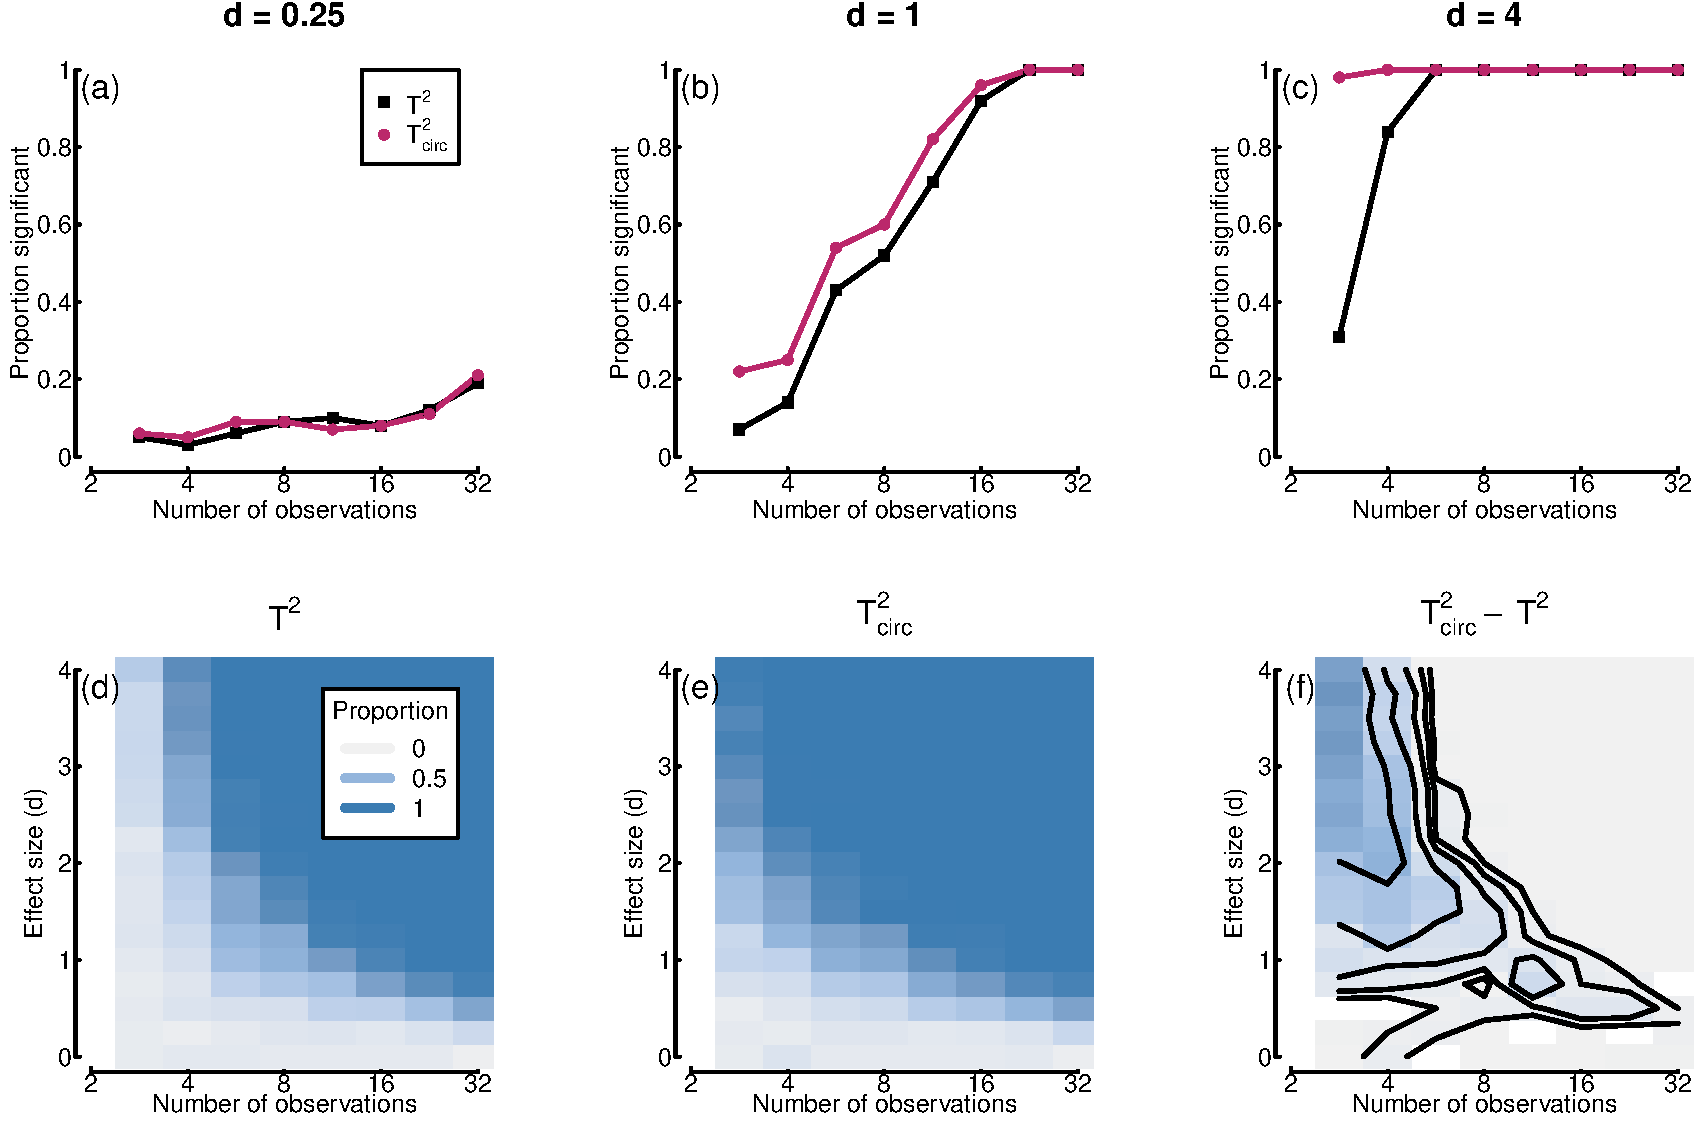
\includegraphics{manuscript_files/figure-latex/powerfig-1} 

}

\caption{Simulations estimating the proportion of significant tests for simulated data with different sample sizes and effect sizes. Panels a-c replicate conditions reported by Victor and Mast (1991). Panels (d) and (e) show a wider range of conditions for each statistic. Panel (f) shows the difference between the two statistics, with contour lines indicating differences of 0.02, 0.05, 0.1, 0.2 and 0.4.}\label{fig:powerfig}
\end{figure}

\hypertarget{limitations-of-t2_circ-when-assumptions-are-violated}{%
\section{\texorpdfstring{Limitations of \(T^2_{circ}\) when assumptions are violated}{Limitations of T\^{}2\_\{circ\} when assumptions are violated}}\label{limitations-of-t2_circ-when-assumptions-are-violated}}

Although \(T^2_{circ}\) can be more sensitive than \(T^2\), this greater sensitivity relies on meeting the test's more stringent assumptions. The two variables must be independent, and of equal variance. These restrictions may hold for some data sets, but it is instructive to ask what happens when they do not. Figure \ref{fig:falsealarms} shows the results of simulations with randomly generated bivariate data in which no signal is present. When the data are uncorrelated and have equal variance (mid-points of the functions in each panel), both tests have the nominal Type I error (false positive) rate of \(\alpha = 0.05\) (dashed line). However, as the data become increasingly correlated (Figure \ref{fig:falsealarms}a), or the variances of the two dependent variables more disparate (Figure \ref{fig:falsealarms}b), the Type I error rate of the \(T^2_{circ}\) statistic (shown in red) increases by almost a factor of 2. In contrast, the \(T^2\) statistic, which explicitly takes account of the covariance matrix (see equation \eqref{eq:t2eq}) shows no increase (black curves).

\begin{figure}
\centering
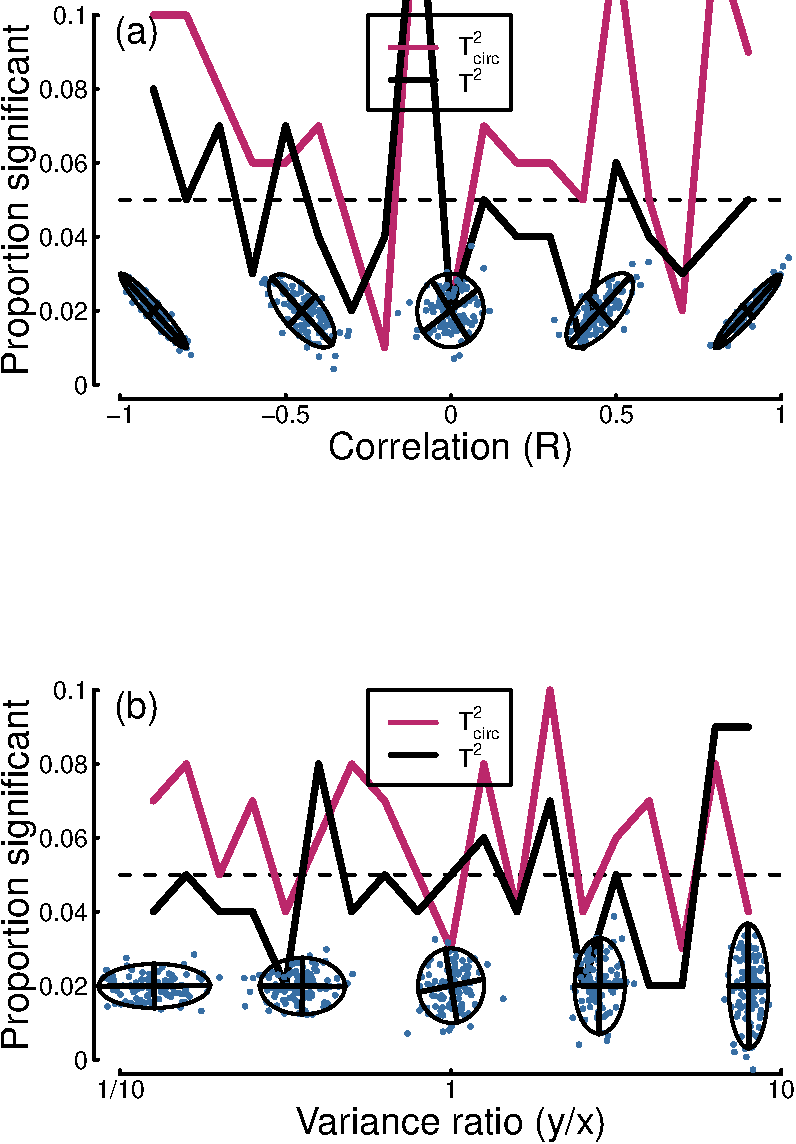
\includegraphics{manuscript_files/figure-latex/falsealarms-1.pdf}
\caption{\label{fig:falsealarms}Simulations showing the Type I error rate for both tests as a function of the correlation between two variables (a) and the ratio of variances (b). Estimates are for 100000 simulations per condition, with N=10 observations. The icons at the foot of each panel show example scatterplots with bounding ellipses and eigenvectors.}
\end{figure}

One possible remedy to control the Type I error rate would be to adjust the alpha level to compensate. However, this will reduce the statistical power of the \(T^2_{circ}\) test, and its advantage over \(T^2\) is relatively marginal in most situations to begin with (see Figure \ref{fig:powerfig}). What is required is a method to objectively assess whether the assumptions of \(T^2_{circ}\) hold, which we develop in the following section.

\hypertarget{a-novel-method-to-test-the-assumptions-of-t2_circ}{%
\section{\texorpdfstring{A novel method to test the assumptions of \(T^2_{circ}\)}{A novel method to test the assumptions of T\^{}2\_\{circ\}}}\label{a-novel-method-to-test-the-assumptions-of-t2_circ}}

Despite the severe consequences of violating the assumptions of the \(T^2_{circ}\) statistic (see Figure \ref{fig:falsealarms}), there is currently no accepted test for those assumptions that could be applied to an empirical data set. Victor and Mast (1991) suggest that their test should be applicable to multiple repetitions of a stimulus condition collected from a single participant, whereas data pooled across multiple participants may be less likely to exhibit independence of the real and imaginary components (see also Pei et al. 2017).

One convenient way to test the assumptions of \(T^2_{circ}\) is to assess the \emph{condition index} of a data set, which describes the ratio of eigenvalues for a cloud of points. The eigenvectors are the major and minor axes of the bounding ellipse (the straight lines in the example icons at the foot of Figure \ref{fig:falsealarms}a,b). Conventionally, the condition index is calculated as the square root of the longest/shortest eigenvector length. For uncorrelated random numbers the distribution of condition indices is positively skewed, with a minimum of 1 (Edelman 1988). This is because two independent samples of numbers from the same underlying distribution will still by chance have unequal eigenvectors. Edelman (1988) provides an equation (Eq 14) for the probability density function of condition indices (x) as a function of sample size (n):

\begin{equation}
\label{eq:edelman1}
pdf = (n-1)2^{n-1}\frac{x^2 - 1}{(x^2 + 1)^n}x^{(n-2)},
\end{equation}

Attempts to validate this by simulation suggest that for small sample sizes (n\textless{}10) a closer approximation is given by:

\begin{equation}
\label{eq:edelman2}
pdf = (n-2)2^{n-2}\frac{x^2 - 1}{(x^2 + 1)^{(n-1)}}x^{(n-3)}
\end{equation}

In Figure \ref{fig:distcomparison}a we show an example distribution derived from the second expression (black curve), the inverse cumulative density function (red curve), and simulations from 100000 random data sets for n=10 (blue shading). The vertical lines show the critical (95\%) threshold for the analytic and simulated results - a ratio lying beyond this threshold can be considered to violate the assumption of either independence or equal variance. Figure \ref{fig:distcomparison}b shows how these thresholds change as a function of the number of observations, and it is clear that the modified expression (red) most closely approximates the simulation results (blue).

\begin{figure}

{\centering 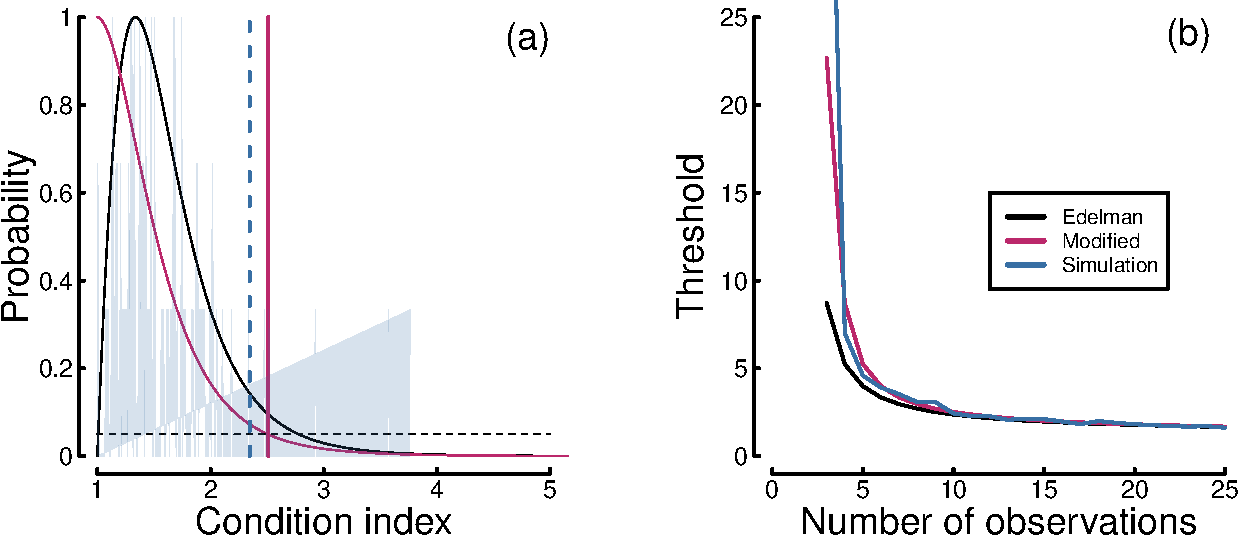
\includegraphics{manuscript_files/figure-latex/distcomparison-1} 

}

\caption{Panel (a) shows the distribution of condition indices derived from Equation 4 (black curve), and by simulation (blue shading), for a sample size of 10 observations. The vertical blue and red lines show the 95 percent thresholds on the curve (where 95 percent of values lie to the left of the line), and the red curve shows the inverse density function. Panel (b) shows how 95 percent thresholds change as a functio of the number of observations.}\label{fig:distcomparison}
\end{figure}

The eigenvalue ratio can be used as a test of the assumptions of \(T^2_{circ}\). If we observe a condition index above the critical threshold for the number of observations then the data set can be said to significantly violate the assumption of equal eigenvalues. Because our modified equation provides an inverse density function (red curve in Figure \ref{fig:distcomparison}a), we can use this to calculate a p-value for the test. If the test is non-significant, one can proceed with \(T^2_{circ}\); if it is significant, \(T^2\) should be used instead. An \emph{R} function implementing this test is included in the project code repository (the \emph{CI.test} function contained in the \emph{CItest.R} script).

\hypertarget{identifying-and-removing-outliers-using-the-mahalanobis-distance}{%
\section{Identifying and removing outliers using the Mahalanobis distance}\label{identifying-and-removing-outliers-using-the-mahalanobis-distance}}

If a data set produces a significant result using the condition index test, this could be due to the presence of one or more outliers. The Mahalanobis distance (Mahalanobis 1936) is a useful metric for identifying such multivariate outliers so that they can be excluded. It calculates the Euclidean distance between each data point and the centroid, and scales it by the variance in the direction of the vector that joins the two points. This means that any correlations in the data set are taken into account when calculating the distance metric, D.

The effectiveness of this approach to outlier exclusion can be assessed by simulation using the condition index test. Figure \ref{fig:outlierplot} shows the proportion of significant condition index tests as a function of the Mahalanobis distance of a single outlier, for a range of sample sizes (curves). In all cases, the functions depart from the Type 1 error rate (\(\alpha\) = 0.05; horizontal dashed line in Figure \ref{fig:outlierplot}) when the Mahalanobis distance exceeds a value around 3. This seems a reasonable heuristic for outlier exclusion, and is the multivariate equivalent of excluding data points more than 3 standard deviations from the mean (note that many implementations of the Mahalanobis distance statistic return \(D^2\), which can be converted to D by taking the square root). Following this heuristic should reduce the likelihood that outliers will invalidate the assumptions of the \(T^2_{circ}\) test.

\begin{figure}

{\centering 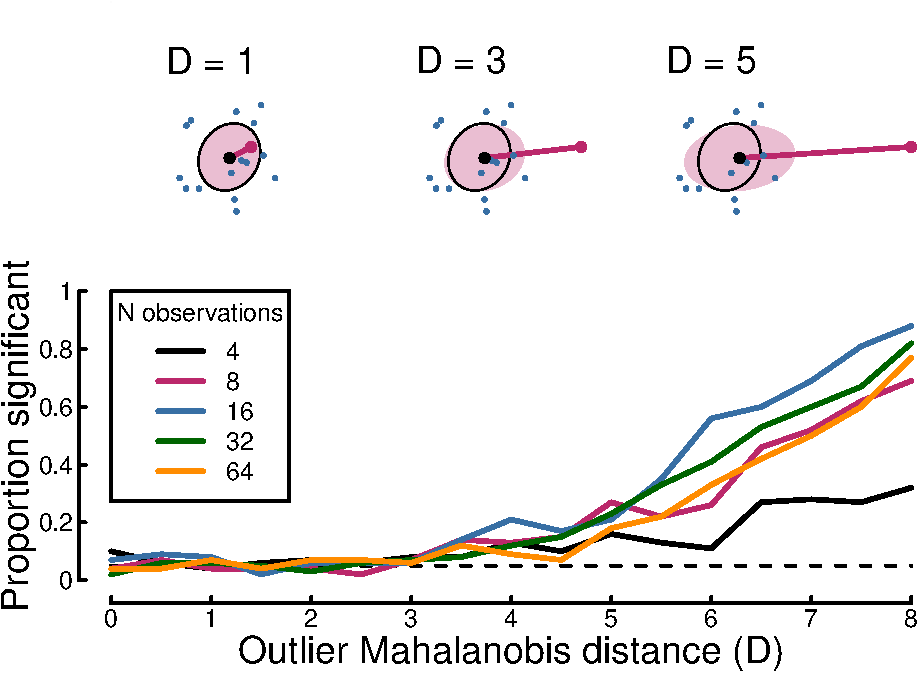
\includegraphics{manuscript_files/figure-latex/outlierplot-1} 

}

\caption{Simulations illustrating the Mahalanobis distance metric, and showing how a single outlier affects the condition index. The upper row shows three example data sets, each with a single outlier shown in red. The outliers have Mahalanobis distances of 1, 3 and 5. The ellipses are calculated with the outlier included (red) and excluded (black), illustrating how the outlier distorts the aspect ratio of the ellipse. The lower plot shows how the proportion of significant condition index tests depends on the outlier distance and the sample size.}\label{fig:outlierplot}
\end{figure}

A variant of the Mahalanobis distance (the pairwise Mahalanobis distance) can also be used to compute a multivariate measure of effect size, equivalent to Cohen's \emph{d} statistic (see e.g. Del Giudice 2009). This is a valuable statistic to include when reporting the results of multivariate tests, and we include an \emph{R} function (\emph{mahalES}) that can be used to calculate it.

\hypertarget{generalising-to-more-than-two-conditions}{%
\section{Generalising to more than two conditions}\label{generalising-to-more-than-two-conditions}}

Many studies involve more than two conditions that need to be compared. Issues with familywise error will quickly become problematic if multiple pairwise \(T^2\) or \(T^2_{circ}\) statistics are calculated. One possibility is to conduct a MANOVA, which takes covariances between dependent variables into account in much the same way as Hotelling's \(T^2\), but permits multiple independent variables with more than two levels. However, if the assumptions of \(T^2_{circ}\) hold for a data set, it might alternatively be possible to extend to logic of the \(T^2_{circ}\) test (Victor and Mast 1991) to the more general case.

The F statistic for a one-way ANOVA is calculated by taking the ratio of the variance explained by the modelled group means to the residual unexplained variance. For multivariate data, the change in group mean would be calculated using the vector distances between the complex means, and the residuals are the vector distances between each data point and its corresponding group mean. For an independent one-way design with \(k\) groups (or conditions) and \(N\) observations per group, the F distribution will have \(2(k-1)\) and \(2((Nk)-k)\) degrees of freedom. The difference between traditional univariate ANOVA is the factor of two scaling, which accounts for the additional degree of freedom for each complex-valued number. A suitable name for such a test might be \({ANOVA}^2_{circ}\), as this reflects the similarity to ANOVA, and the extension of the logic of \(T^2_{circ}\) (an alternative name might be \(MANOVA_{circ}\), however this feels less appropriate given that many of the key features of MANOVA are absent).

Figure \ref{fig:powerfig2} shows simulations analogous to those in Figure \ref{fig:powerfig} for a one-way design with three levels. MANOVA is directly compared to the \({ANOVA}^2_{circ}\) statistic across a range of effect sizes and sample sizes. Just as for the one-sample statistics, the advantages of \({ANOVA}^2_{circ}\) are particularly apparent for small sample sizes, and larger effect sizes (Figure \ref{fig:powerfig2}f).

\begin{figure}

{\centering 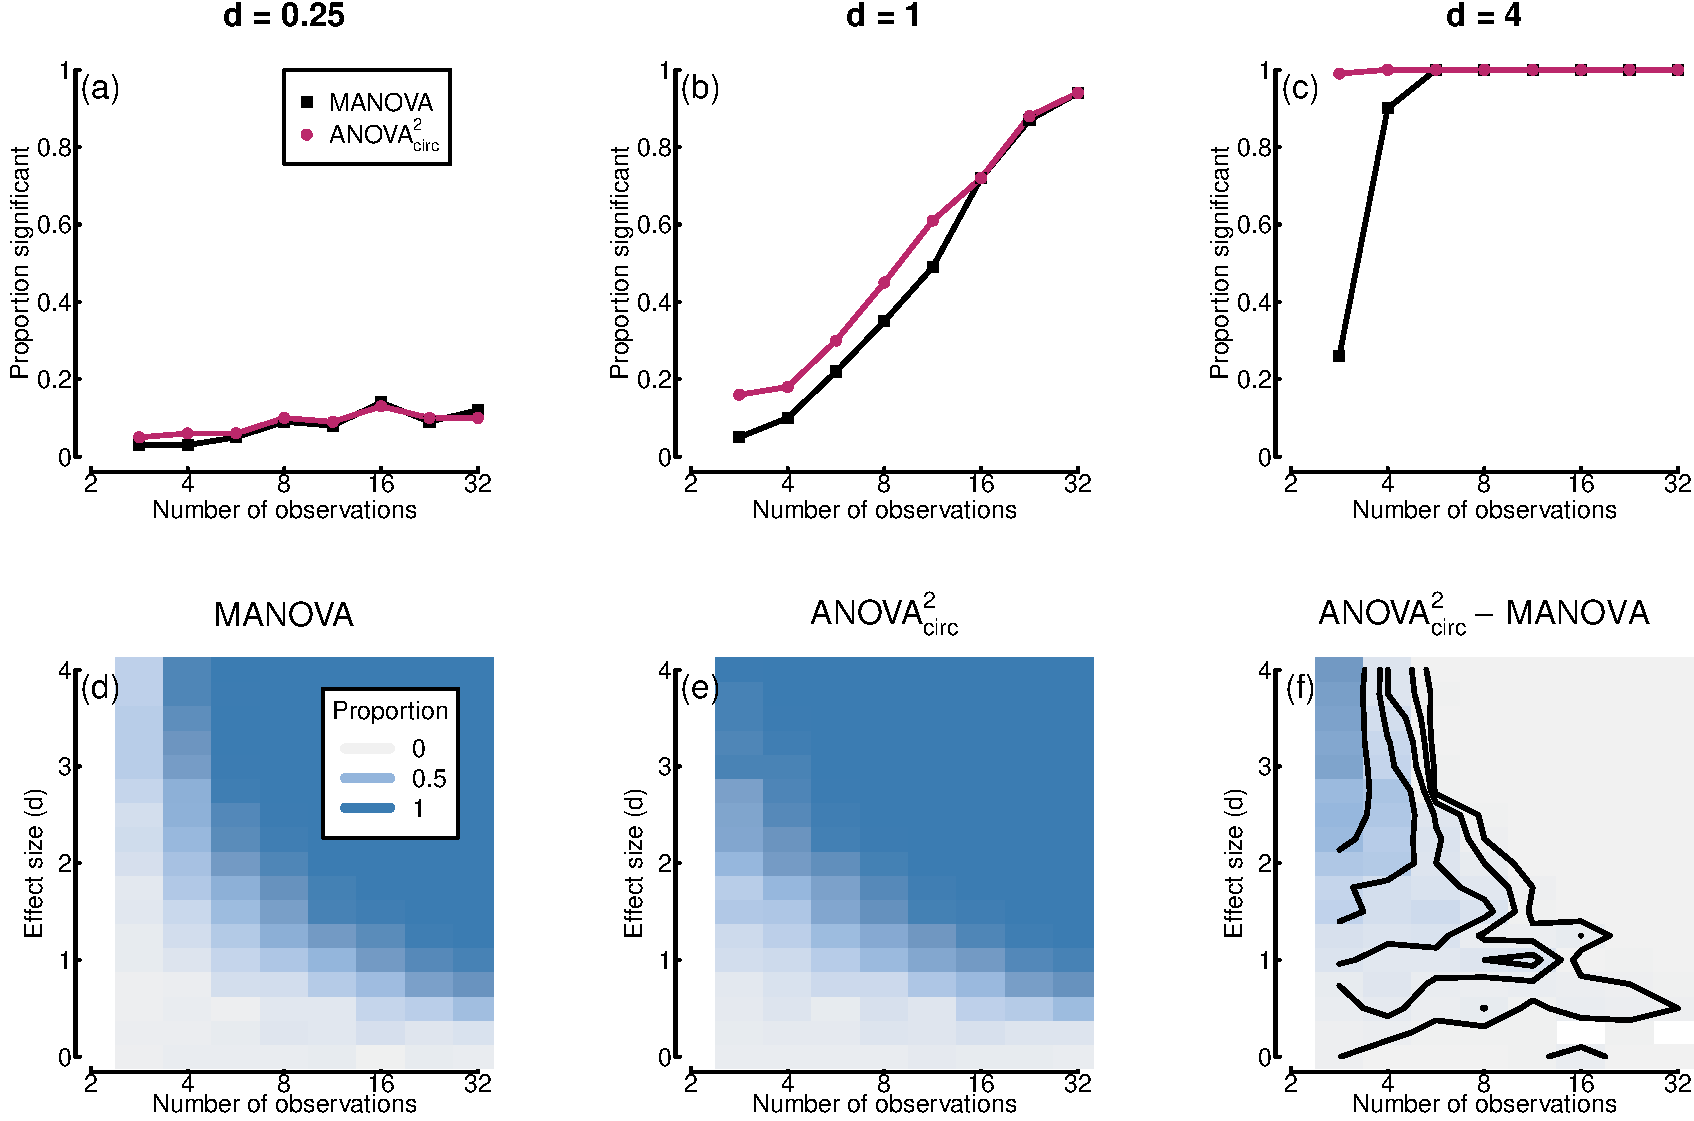
\includegraphics{manuscript_files/figure-latex/powerfig2-1} 

}

\caption{Simulations comparing the sensitivity of MANOVA and ANOVA2circ. The format mirrors that of Figure 2. In these simulations, there were three conditions, with the signal being added to one condition.}\label{fig:powerfig2}
\end{figure}

Following \({ANOVA}^2_{circ}\), one could calculate \(T^2_{circ}\) statistics to make post-hoc pairwise comparisons between conditions, providing that standard Bonferroni corrections are applied. Univariate ANOVAs on the real and imaginary components are unlikely to be informative, as the relative magnitudes depend on stimulus phase (which is arbitrary). A repeated measures version of \({ANOVA}^2_{circ}\) has also been implemented following the same logic. The project repository contains \emph{R} scripts for both of these functions.

\hypertarget{deciding-which-test-to-run}{%
\section{Deciding which test to run}\label{deciding-which-test-to-run}}

The flowchart in Figure \ref{fig:flowchart} contains a proposed decision structure for the analysis of periodic data. Initially, data for each condition should be tested against the expected distribution of eigenvalue ratios. Comparisons with one or two conditions should be tested with the \(T^2_{circ}\) statistic if the eigenvalue ratios are consistent with circularity, and the \(T^2\) statistic if not. Comparisons with more than two conditions should be tested with the \(ANOVA^2_{circ}\) statistic if the eigenvalue ratios are consistent with circularity, or a MANOVA if not. Some MANOVA implementations cannot deal with random factors (repeated measures) in complex factorial designs. In \emph{R}, the \emph{Manova} function from the \emph{car} package appears to be capable of the necessary calculations, as does the commercial software package SPSS.

\begin{figure}

{\centering 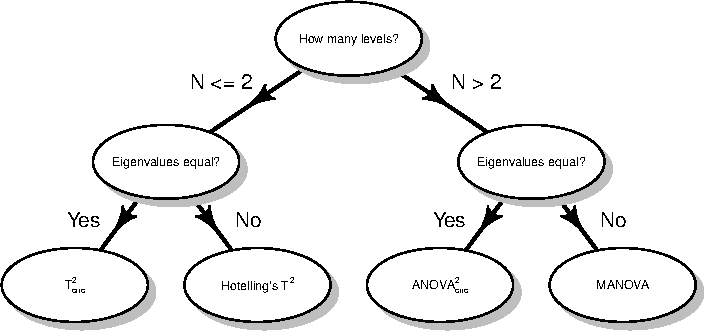
\includegraphics{manuscript_files/figure-latex/flowchart-1} 

}

\caption{Flowchart illustrating how one might decide which test to conduct for a given data set, based on the study design and the outcome of the condition index test.}\label{fig:flowchart}
\end{figure}

\hypertarget{applying-these-methods-to-empirical-data-sets}{%
\section{Applying these methods to empirical data sets}\label{applying-these-methods-to-empirical-data-sets}}

Having developed some novel tools for the analysis of periodic data, in the following sections we demonstrate them using two different publicly available empirical data sets. The first study recorded responses to auditory and optogenetic stimulation in mice. The second study measured visual responses to flickering grating patterns in humans. These cases provide examples of how the results of the tests described above might be appropriately reported.

\hypertarget{mouse-auditory-and-optogenetic-steady-state-data}{%
\subsection{Mouse auditory and optogenetic steady-state data}\label{mouse-auditory-and-optogenetic-steady-state-data}}

Hwang et al. (2019, 2020) measured steady-state responses using implanted scalp electrodes in 6 mice. The mice had previously been given a targeted virus that made parvalbumin neurons in their basal forebrain responsive to specific wavelengths of light, delivered through an optical fiber (a technique called optogenetics). SSVEPs were recorded from 36 electrodes for 1 second epochs of 40 Hz auditory stimulation, and various schedules of optogenetic stimulation (including at 40 Hz). The data set is described more fully by Hwang et al. (2020), and was downloaded from: \url{https://doi.gin.g-node.org/10.12751/g-node.e5tyek/}.

Figure \ref{fig:mousedata}a shows Fourier amplitude spectra at two frontal electrodes (marked black in the insets) for auditory stimulation (red) and optogenetic stimulation (blue), each at 40 Hz. There is a clear frequency-locked signal with approximately equal amplitude for each stimulation modality. Indeed, a paired t-test on the amplitudes reveals no significant difference (t=0.84, df=5, p=0.44). However, inspection of the complex Fourier components for each condition suggests evidence of a phase difference between the two modalities (see Figure \ref{fig:mousedata}b). The condition index test was non-significant for both conditions (sound: CI = 1.59, \emph{p} = 0.66; light: CI = 1.69, \emph{p} = 0.59), so a paired-samples \(T^2_{circ}\) test was conducted. This revealed a significant difference between conditions (\(T^2_{circ}\) = 1.39, \(F_{(2,10)}\) = 8.32, \emph{p} = 0.007) with an effect size of D = 1.02. This demonstrates that both sound and (optogenetic) light are able to entrain neural responses - the original study by Hwang et al. (2019) went on to explore interactions between these two signals.

\begin{figure}

{\centering 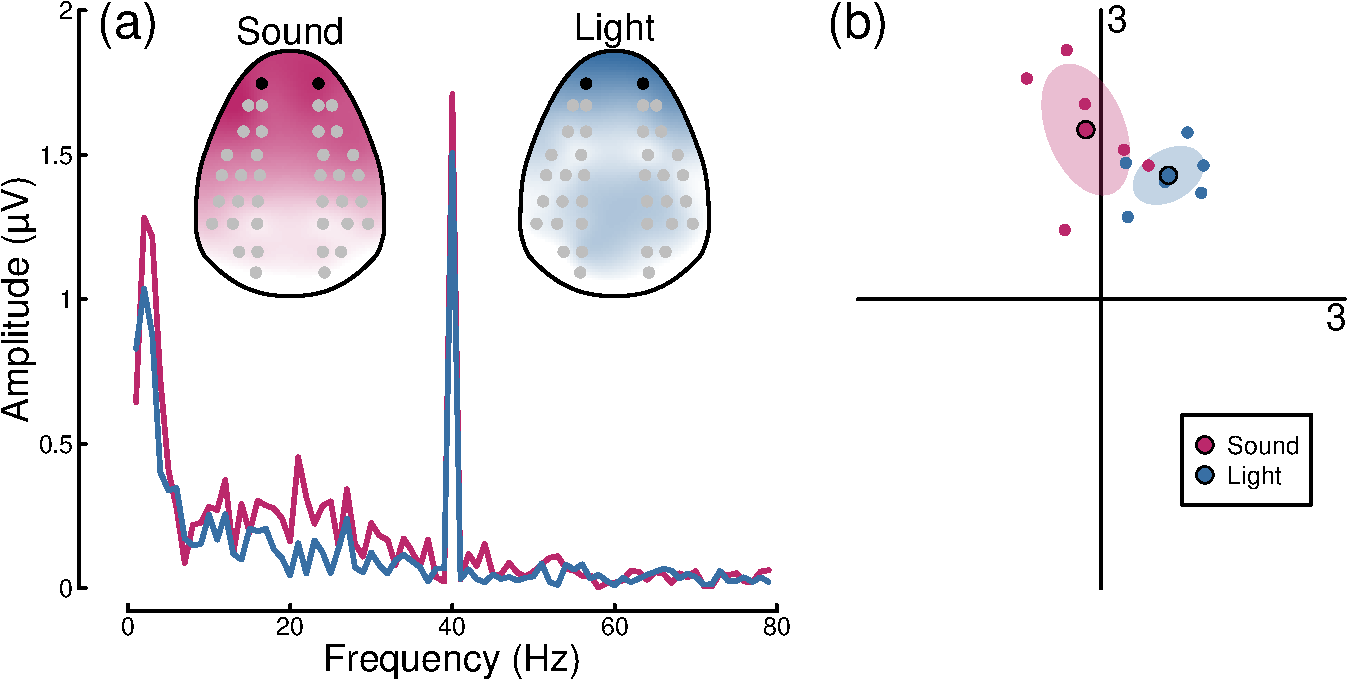
\includegraphics{manuscript_files/figure-latex/mousedata-1} 

}

\caption{Summary of mouse steady-state responses to 40 Hz stimulation. Panel (a) shows the Fourier amplitude spectrum with inset scalp plots for sound (red) and light (blue) stimulation, averaged across repetitions and individuals. Panel (b) shows complex (x = real, y = imaginary) Fourier components for 6 individual mice (small points) and their average (large points) for both conditions.}\label{fig:mousedata}
\end{figure}

\hypertarget{human-visual-steady-state-data}{%
\subsection{Human visual steady-state data}\label{human-visual-steady-state-data}}

Vilidaite et al. (2018) measured visual responses to flickering grating stimuli in a large sample of 100 adults. Each participant completed a series of 11-second trials, in which stimuli of different contrasts flickered at 7Hz (on-off sinusoidal flicker). Responses were strongest at occipital electrodes over visual cortex (see upper row of Figure \ref{fig:humanSSVEP}), were well-isolated in the Fourier domain, and increased with stimulus contrast. For this analysis, we took responses from electrode \emph{Oz} at the occipital pole (black points in the upper row of Figure \ref{fig:humanSSVEP}), averaged across repetition for each participant. Each condition included some outlier points with Mahalanobis distances exceeding 3, marked red in the lower row of Figure \ref{fig:humanSSVEP}. Any participant that contributed at least one outlier was excluded, leaving a total of 89 participants for the main analysis.

\begin{figure}

{\centering 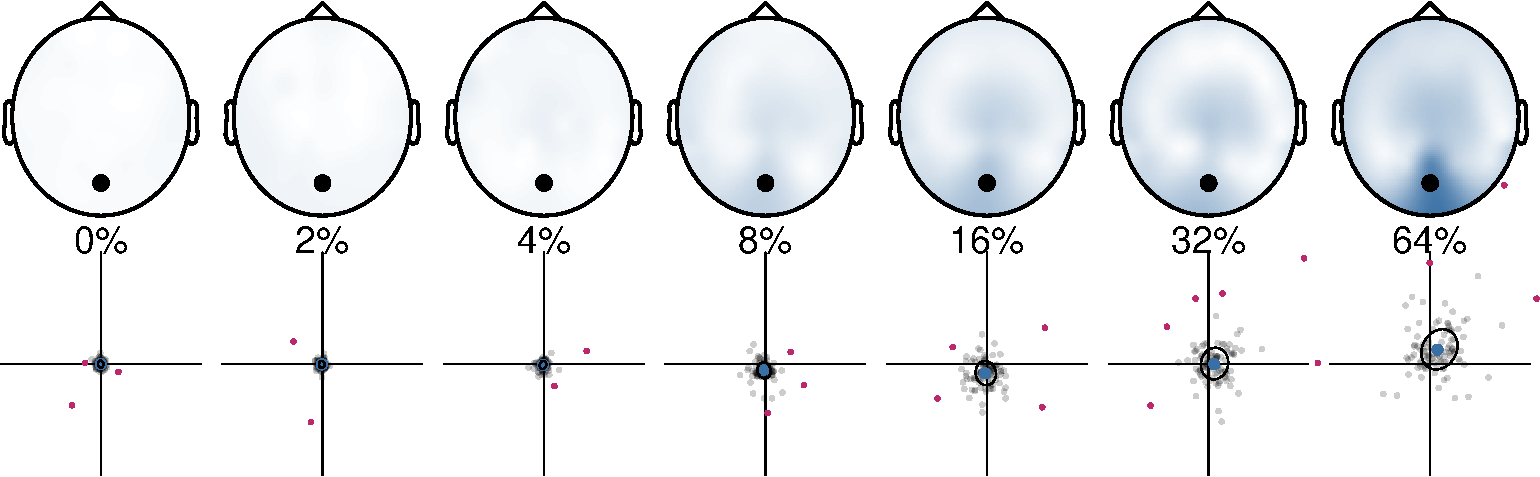
\includegraphics{manuscript_files/figure-latex/humanSSVEP-1} 

}

\caption{Summary of human SSVEP data. Upper row shows scalp distributions of Fourier amplitudes at 7Hz for stimuli of increasing contrasts (blue shading indicates higher amplitudes). Lower row shows scatterplots of complex (x = real, y = imaginary) Fourier components for 100 participants per condition, from electrode Oz (black point). Red points are outliers with Mahalanobis distances exceeding 3, and blue points mark the centroids.}\label{fig:humanSSVEP}
\end{figure}

With the outlier points removed, all seven conditions resulted in non-significant condition index tests (largest CI = 1.2, all \emph{p} \textgreater{} 0.19). A repeated measures \(ANOVA^2_{circ}\) test was conducted, revealing a significant effect of stimulus contrast (\(F_{(12,1056)}\) = 38.9, p \textless{} 0.001). Pairwise \(T^2_{circ}\) statistics comparing the baseline (0\% contrast) condition to each subsequent condition (Bonferroni corrected for 6 tests to \(\alpha = 0.08\)) revealed significant differences at 8\% contrast (\(T^2_{circ}\) = 0.32, \(F_{(2,176)}\) = 28.4, D = 0.13, \emph{p} \textless{} 0.001), 16\% contrast (\(T^2_{circ}\) = 0.28, \(F_{(2,176)}\) = 25.3, D = 0.19, \emph{p} \textless{} 0.001), 32\% contrast (\(T^2_{circ}\) = 0.10, \(F_{(2,176)}\) = 8.5, D = 0.14, \emph{p} \textless{} 0.001) and 64\% contrast (\(T^2_{circ}\) = 0.34, \(F_{(2,176)}\) = 35.3, D = 0.33, \emph{p} \textless{} 0.001). The study by Vilidaite et al. (2018) compared SSVEP responses between individuals with and without autism, as well as in a \emph{Drosophila} genetic model of developmental disorders. The raw data are available at: \url{http://dx.doi.org/10.17605/OSF.IO/Y4N5K}.

\hypertarget{further-considerations}{%
\section{Further considerations}\label{further-considerations}}

It is worth pointing out that the statistical tests discussed in this paper are applicable only when the signal phase is expected to be consistent across observations. This is the case for most paradigms in which the nervous system is driven by a periodic stimulus. However, they are less obviously applicable to the analysis of endogenous neural oscillations and brain rhythms (Berger 1929; Buzsáki and Draguhn 2004), which will typically have random phase and broader bandwidths in the Fourier domain: other analysis methods have been developed for such signals (e.g. Canolty and Knight 2010). When phases are consistent across repetitions, greater statistical power can be obtained by coherently averaging across repetitions to obtain a participant-level average (Baker et al. 2020). This practice is also necessary in order to use the multivariate methods discussed here, as the alternative is to discard the phase information and average amplitudes instead, rendering the data univariate.

The present paper has focussed on the Frequentist statistical tradition. However there are many advantages to the Bayesian approach, in which one can make direct quantitative comparisons of the evidence supporting both the experimental and null hypotheses. Subject to determining appropriate priors, Bayes factor scores might be calculated for all of the statistics considered here, much as has been done previously for univariate T-tests (Rouder et al. 2009). However this is a non-trivial undertaking, and is beyond the scope of the current paper.

Another possibility is to use machine learning techniques such as multivariate pattern analysis (MVPA) to analyse periodic data. This involvess training a classifier algorithm to distinguish between two (or more) experimental conditions or states, and then assessing classifier accuracy on fresh data. If different conditions produce distinct patterns of neural response, then classifier accuracy will be above chance. Such methods have been hugely influential in the fMRI literature, and for analysing event-related potential data collected using EEG or MEG. However, they have not been widely applied to steady-state data (though see West et al. (2015) for an example). In principle, the real and imaginary Fourier components can be treated as separate dependent variables, along with different recording locations and/or frequencies. This approach has the potential to offer sensitive, high-powered statistical tests that circumvent many of the shortcomings associated with parametric statistics.

Even when statistics are conducted using both the real and imaginary Fourier components, it is still typical to visualise the mean amplitudes. Several approaches to calculating appropriate error bars have been proposed. For example, Pei et al. (2017) suggest calculating the nearest and farthest points from the origin on the bounding ellipse, and using these to derive standard errors for the amplitude. This approach is somewhat computationally demanding, though we have implemented an \emph{R} function to calculate error bars using this method. However, we feel that bootstrap resampling offers a powerful and general alternative for calculating 95\% confidence intervals on amplitudes. This is achieved by resampling the complex data (with replacement) and calculating a resampled complex mean. The amplitude is then derived for this resampled mean, and the procedure repeated a large number of times (1000 or 10000 repetitions is typical) to build up a population of resampled amplitudes. Upper and lower 95\% confidence intervals on the amplitude can then be taken at appropriate quantiles of this population.

\hypertarget{general-recommendations-for-analysing-periodic-data}{%
\section{General recommendations for analysing periodic data}\label{general-recommendations-for-analysing-periodic-data}}

The simulations reported here allow us to make several recommendations for how periodic data should be analysed. Multivariate statistics should be used for phase-locked Fourier data instead of univariate statistics such as T-tests and ANOVA. This avoids problems from distributions of amplitudes violating the test assumptions, and also provides a sensitivity benefit from the inclusion of phase information. Outliers should be removed when they have a Mahalanobis distance exceeding 3, and the pairwise Mahanalobis distance reported as a measure of effect size. For sample sizes of N \textless{} 32, the \(T^2_{circ}\) and \(ANOVA^2_{circ}\) statistics can be used if the condition index test is non-significant for all conditions. Alternatively, the \(T^2\) or MANOVA statistics should be used when these conditions are not met. The greater power afforded by these tests should in general lead to more accurate statistical inferences when analysing periodic data.

\hypertarget{references}{%
\section*{References}\label{references}}
\addcontentsline{toc}{section}{References}

\hypertarget{refs}{}
\leavevmode\hypertarget{ref-Afsari2014}{}%
Afsari, Farinaz, Kenneth V Christensen, Garrick Paul Smith, Morten Hentzer, Olivia M Nippe, Christopher J H Elliott, and Alex R Wade. 2014. ``Abnormal Visual Gain Control in a Parkinson's Disease Model.'' \emph{Hum Mol Genet} 23 (17): 4465--78. \url{https://doi.org/10.1093/hmg/ddu159}.

\leavevmode\hypertarget{ref-Baker2020}{}%
Baker, D.H., G. Vilidaite, F.A. Lygo, A.K. Smith, T.R. Flack, A.D. Gouws, and T.J. Andrews. 2020. ``Power Contours: Optimising Sample Size and Precision in Experimental Psychology and Human Neuroscience.'' \emph{Psychological Methods}. \url{https://doi.org/10.1037/met0000337}.

\leavevmode\hypertarget{ref-Berger1929}{}%
Berger, H. 1929. ``Über Das Elektrenkephalogramm Des Menschen.'' \emph{Archiv F. Psychiatrie} 87: 527--70. \url{https://doi.org/10.1007/BF01797193}.

\leavevmode\hypertarget{ref-Braddick1986}{}%
Braddick, O J, J Wattam-Bell, and J Atkinson. 1986. ``Orientation-Specific Cortical Responses Develop in Early Infancy.'' \emph{Nature} 320 (6063): 617--9. \url{https://doi.org/10.1038/320617a0}.

\leavevmode\hypertarget{ref-Buzsaki2004}{}%
Buzsáki, György, and Andreas Draguhn. 2004. ``Neuronal Oscillations in Cortical Networks.'' \emph{Science} 304 (5679): 1926--9. \url{https://doi.org/10.1126/science.1099745}.

\leavevmode\hypertarget{ref-Canolty2010}{}%
Canolty, Ryan T, and Robert T Knight. 2010. ``The Functional Role of Cross-Frequency Coupling.'' \emph{Trends Cogn Sci} 14 (11): 506--15. \url{https://doi.org/10.1016/j.tics.2010.09.001}.

\leavevmode\hypertarget{ref-Cohen1988}{}%
Cohen, J. 1988. \emph{Statistical Power Analysis for the Behavioral Sciences}. Lawrence Erlbaum, Hillsdale, New Jersey.

\leavevmode\hypertarget{ref-Giudice2009}{}%
Del Giudice, M. 2009. ``On the Real Magnitude of Psychological Sex Differences.'' \emph{Evolutionary Psychology} 7: 264--79. \url{https://doi.org/10.1177/147470490900700209}.

\leavevmode\hypertarget{ref-Edelman1988}{}%
Edelman, Alan. 1988. ``Eigenvalues and Condition Numbers of Random Matrices.'' \emph{SIAM Journal on Matrix Analysis and Applications} 9 (4): 543--60. \url{https://doi.org/10.1137/0609045}.

\leavevmode\hypertarget{ref-Engel1994}{}%
Engel, S A, D E Rumelhart, B A Wandell, A T Lee, G H Glover, E J Chichilnisky, and M N Shadlen. 1994. ``FMRI of Human Visual Cortex.'' \emph{Nature} 369 (6481): 525. \url{https://doi.org/10.1038/369525a0}.

\leavevmode\hypertarget{ref-Enroth-Cugell1966}{}%
Enroth-Cugell, C, and J G Robson. 1966. ``The Contrast Sensitivity of Retinal Ganglion Cells of the Cat.'' \emph{J Physiol} 187 (3): 517--52. \url{https://doi.org/10.1113/jphysiol.1966.sp008107}.

\leavevmode\hypertarget{ref-Gray2020}{}%
Gray, Katie L H, Tessa R Flack, Miaomiao Yu, Freya A Lygo, and Daniel H Baker. 2020. ``Nonlinear Transduction of Emotional Facial Expression.'' \emph{Vision Res} 170 (May): 1--11. \url{https://doi.org/10.1016/j.visres.2020.03.004}.

\leavevmode\hypertarget{ref-Hotelling1931}{}%
Hotelling, H. 1931. ``The Generalization of Student's Ratio.'' \emph{The Annals of Mathematical Statistics} 2 (3). Institute of Mathematical Statistics: 360--78. \url{http://www.jstor.org/stable/2957535}.

\leavevmode\hypertarget{ref-Hwang2019}{}%
Hwang, Eunjin, Ritchie E Brown, Bernat Kocsis, Tae Kim, James T McKenna, James M McNally, Hio-Been Han, and Jee Hyun Choi. 2019. ``Optogenetic Stimulation of Basal Forebrain Parvalbumin Neurons Modulates the Cortical Topography of Auditory Steady-State Responses.'' \emph{Brain Struct Funct} 224 (4): 1505--18. \url{https://doi.org/10.1007/s00429-019-01845-5}.

\leavevmode\hypertarget{ref-Hwang2020}{}%
Hwang, Eunjin, Hio-Been Han, Jung Young Kim, and Jee Hyun Choi. 2020. ``High-Density Eeg of Auditory Steady-State Responses During Stimulation of Basal Forebrain Parvalbumin Neurons.'' \emph{Sci Data} 7 (1): 288. \url{https://doi.org/10.1038/s41597-020-00621-z}.

\leavevmode\hypertarget{ref-Liu-Shuang2014}{}%
Liu-Shuang, Joan, Anthony M Norcia, and Bruno Rossion. 2014. ``An Objective Index of Individual Face Discrimination in the Right Occipito-Temporal Cortex by Means of Fast Periodic Oddball Stimulation.'' \emph{Neuropsychologia} 52 (January): 57--72. \url{https://doi.org/10.1016/j.neuropsychologia.2013.10.022}.

\leavevmode\hypertarget{ref-Mahalanobis1936}{}%
Mahalanobis, P.C. 1936. ``On the Generalised Distance in Statistics.'' \emph{Proceedings of the National Academy of Sciences of India} 2: 49--55.

\leavevmode\hypertarget{ref-Morrone1987}{}%
Morrone, M C, D C Burr, and H D Speed. 1987. ``Cross-Orientation Inhibition in Cat Is Gaba Mediated.'' \emph{Exp Brain Res} 67 (3): 635--44. \url{https://doi.org/10.1007/BF00247294}.

\leavevmode\hypertarget{ref-Nakayama1982}{}%
Nakayama, K, and M Mackeben. 1982. ``Steady State Visual Evoked Potentials in the Alert Primate.'' \emph{Vision Res} 22 (10): 1261--71. \url{https://doi.org/10.1016/0042-6989(82)90138-9}.

\leavevmode\hypertarget{ref-Norcia2015}{}%
Norcia, Anthony M, L Gregory Appelbaum, Justin M Ales, Benoit R Cottereau, and Bruno Rossion. 2015. ``The Steady-State Visual Evoked Potential in Vision Research: A Review.'' \emph{J Vis} 15 (6): 4. \url{https://doi.org/10.1167/15.6.4}.

\leavevmode\hypertarget{ref-Pei2017}{}%
Pei, Francesca, Stefano Baldassi, Jeffrey J Tsai, Holly E Gerhard, and Anthony M Norcia. 2017. ``Development of Contrast Normalization Mechanisms During Childhood and Adolescence.'' \emph{Vision Res} 133 (April): 12--20. \url{https://doi.org/10.1016/j.visres.2016.03.010}.

\leavevmode\hypertarget{ref-Porciatti1990}{}%
Porciatti, V, G Fontanesi, A Raffaelli, and P Bagnoli. 1990. ``Binocularity in the Little Owl, Athene Noctua. II. Properties of Visually Evoked Potentials from the Wulst in Response to Monocular and Binocular Stimulation with Sine Wave Gratings.'' \emph{Brain Behav Evol} 35 (1): 40--48. \url{https://doi.org/10.1159/000115855}.

\leavevmode\hypertarget{ref-Rees1986}{}%
Rees, A, G G Green, and R H Kay. 1986. ``Steady-State Evoked Responses to Sinusoidally Amplitude-Modulated Sounds Recorded in Man.'' \emph{Hear Res} 23 (2): 123--33. \url{https://doi.org/10.1016/0378-5955(86)90009-2}.

\leavevmode\hypertarget{ref-Regan1966}{}%
Regan, D. 1966. ``Some Characteristics of Average Steady-State and Transient Responses Evoked by Modulated Light.'' \emph{Electroencephalogr Clin Neurophysiol} 20 (3): 238--48. \url{https://doi.org/10.1016/0013-4694(66)90088-5}.

\leavevmode\hypertarget{ref-Rouder2009}{}%
Rouder, Jeffrey N, Paul L Speckman, Dongchu Sun, Richard D Morey, and Geoffrey Iverson. 2009. ``Bayesian T Tests for Accepting and Rejecting the Null Hypothesis.'' \emph{Psychon Bull Rev} 16 (2): 225--37. \url{https://doi.org/10.3758/PBR.16.2.225}.

\leavevmode\hypertarget{ref-Sereno1995}{}%
Sereno, M I, A M Dale, J B Reppas, K K Kwong, J W Belliveau, T J Brady, B R Rosen, and R B Tootell. 1995. ``Borders of Multiple Visual Areas in Humans Revealed by Functional Magnetic Resonance Imaging.'' \emph{Science} 268 (5212): 889--93. \url{https://doi.org/10.1126/science.7754376}.

\leavevmode\hypertarget{ref-Snyder1992}{}%
Snyder, A Z. 1992. ``Steady-State Vibration Evoked Potentials: Descriptions of Technique and Characterization of Responses.'' \emph{Electroencephalogr Clin Neurophysiol} 84 (3): 257--68. \url{https://doi.org/10.1016/0168-5597(92)90007-x}.

\leavevmode\hypertarget{ref-Spitschan2014}{}%
Spitschan, Manuel, Sandeep Jain, David H Brainard, and Geoffrey K Aguirre. 2014. ``Opponent Melanopsin and S-Cone Signals in the Human Pupillary Light Response.'' \emph{Proc Natl Acad Sci U S A} 111 (43): 15568--72. \url{https://doi.org/10.1073/pnas.1400942111}.

\leavevmode\hypertarget{ref-Victor1991}{}%
Victor, J D, and J Mast. 1991. ``A New Statistic for Steady-State Evoked Potentials.'' \emph{Electroencephalogr Clin Neurophysiol} 78 (5): 378--88. \url{https://doi.org/10.1016/0013-4694(91)90099-p}.

\leavevmode\hypertarget{ref-Vilidaite2018}{}%
Vilidaite, Greta, Anthony M Norcia, Ryan J H West, Christopher J H Elliott, Francesca Pei, Alex R Wade, and Daniel H Baker. 2018. ``Autism Sensory Dysfunction in an Evolutionarily Conserved System.'' \emph{Proc Biol Sci} 285 (1893): 20182255. \url{https://doi.org/10.1098/rspb.2018.2255}.

\leavevmode\hypertarget{ref-West2015}{}%
West, Ryan J H, Christopher J H Elliott, and Alex R Wade. 2015. ``Classification of Parkinson's Disease Genotypes in Drosophila Using Spatiotemporal Profiling of Vision.'' \emph{Sci Rep} 5 (November): 16933. \url{https://doi.org/10.1038/srep16933}.

\end{document}
